\documentclass[a4paper, 12pt, oneside]{book}
\usepackage{amssymb}
\usepackage{amsmath}
\usepackage[english]{babel}
\usepackage{xcolor}
\usepackage{graphicx}
\usepackage[noprint,thirtytwo,twouparticle]{booklet}

\def\hrulefill{\leavevmode\leaders\hrule height 0.1pt\hfill\kern 0pt}

\newcommand\Linepage[1][0.3in]{% Change to suit
    %\color{gray!50}
  \vbox to \dimexpr\textheight-\pagetotal-#1\relax {% Let TeX do the work...
    \leaders\hbox to \linewidth{\rule{0pt}{#1}\hrulefill}\vfil
  }%
}
\newcommand{\mypage}{\newpage{\Linepage}\newpage}
\newcommand{\mydate}[1]{\noindent\emph{#1}}
\newcommand{\mytime}[1]{\hfill\emph{#1}\vspace{0.3cm}\\}
\newcommand{\myauthor}[1]{\noindent{\large \bf #1}}
\newcommand{\myaffiliation}[1]{\large (#1)\\}
\newcommand{\mytitle}[1]{\noindent\begin{center}{\Large\it #1}\end{center}}
\newenvironment{myabstract}{}{\par\Linepage}

\begin{document}
\pagestyle{empty}
\setpdftargetpages  % if you use pdflatex
\begin{center}
    \mbox{}
    \vfill
    \Large\bf
    Calculus of Variations\\ and \\Partial Differential Equations\\
    \vskip 0.5cm
    \large \textbf{Workshop in honour of Luigi Ambrosio's 60th birthday}
    \vskip 0.5cm
    \normalsize
    \textbf{June 12-16, 2023}
    \vskip 0.5cm
    \textbf{Aula Magna Università di Pisa}\\ 
    \textbf{Largo Bruno Pontecorvo 5}    
    
    \vfill

    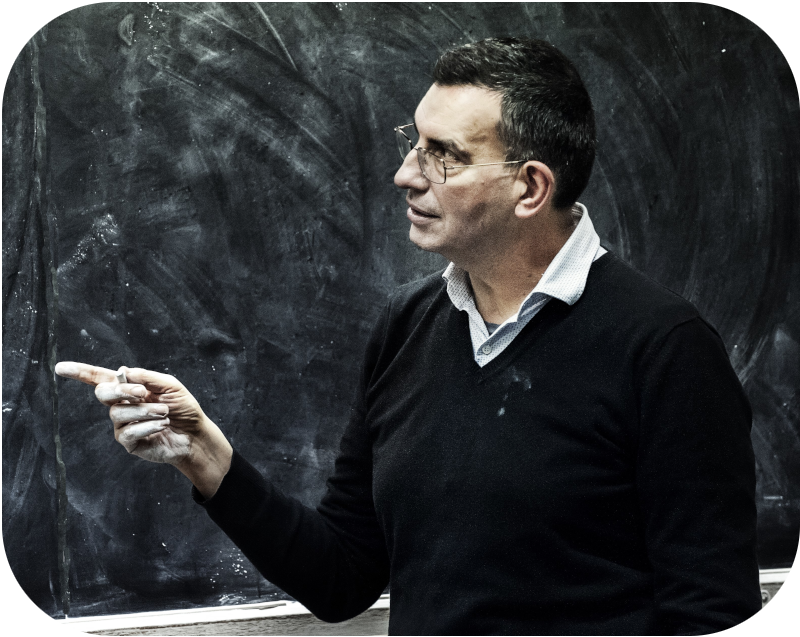
\includegraphics[width=0.5\textwidth]{ambrosio.png}

    \vfill

    \begin{tabular}{lcl}
    \includegraphics*[height=1.8cm]{matematica_dx_nero.pdf}
    & \hspace{2cm}&
    \includegraphics*[height=2cm]{marchio_unipi_orizz_black.png}
    \\
    \mbox{\hspace{3mm}}\includegraphics*[height=2cm]{Sns-Scuola-Normale-Superiore-Pisa-black.png}
    & &
    \includegraphics*[height=2.2cm]{logo_DIMAI_negativo-1-768x384.png}
    \end{tabular}
  \end{center}
    
\newpage
{\Linepage}
%{\Linepage}
\newpage
\begin{center}
\textbf{\large Timetable, June 12-16}
\vskip 0.5cm
\begin{tabular}{|r|ccccc|}
\hline
\it   & monday & tuesday & wednesday & thursday & friday \\
\hline
\it 9:00  & -- & \bf De Philippis & \bf Cabré & \bf Fonseca & \bf Dal Maso \\ 
\it 9:30  & \it welcome & $\vert$ & $\vert$ & $\vert$ & $\vert$ \\ 
\it 10:00 & \bf Figalli & \it break & \it break & \it break & \it break \\
\it 10:30 & $\vert$ & \bf Fusco & \bf Pallara & \bf Gigli & \bf Cannarsa \\
\it 11:00 & \it break & $\vert$ & $\vert$ & $\vert$ & $\vert$ \\
\it 11:30 & \bf Savaré & \bf Garroni & \bf Mondino & \bf Buttazzo & \bf Brenier \\
          & $\vert$ & $\vert$ & $\vert$ & $\vert$ & $\vert$ \\
\hline
\it 13:30 & \it lunch & \it lunch & \it lunch & \it lunch & \it lunch \\
\hline
\it 14:30 & \bf Braides & \bf \bf Mantegazza & \bf Serra & \bf Trevisan & \\
          & $\vert$ & $\vert$ & \bf Cassano & $\vert$ & \\
\it 15:30 & \it break & \it break & \it break & \it break & \\
\it 16:00 & \bf Fornasier & \bf \bf Alberti & \bf Masnou & \bf Honda & \\
 & $\vert$ & $\vert$ & $\vert$ & $\vert$ & \\
\hline
\end{tabular}
\end{center}
{\Linepage}

\mypage
\mydate{Monday, 12 June 2023}
\mytime{10:00}
\myauthor{FIGALLI, Alessio}
\myaffiliation{ETH Zürich}
\mytitle{Free boundary regularity for the obstacle problem}
\begin{myabstract}   
The classical obstacle problem consists of finding the equilibrium position of an elastic membrane whose boundary is held fixed and constrained to lie above a given obstacle. By classical results of Caffarelli, the free boundary is smooth outside a set of singular points. However, explicit examples show that the singular set could be, in general, as large as the regular set. This talk aims to introduce this beautiful problem and describe some classical and recent results on the regularity of the free boundary.
\end{myabstract}


\mypage
\mydate{Monday, 12 June 2023}
\mytime{11:30}
\myauthor{SAVARÉ, Giuseppe}
\myaffiliation{Università Bocconi, Milano}
\mytitle{Evolution of probability measures:\\beyond gradient flows}
\begin{myabstract}
The theory of contraction semigroups in the Wasserstein space of Euclidean probability measures generated by displacement convex functionals is well understood: the variational approach relies on convergence estimates on the Jordan-Kinderlehrer-Otto
Minimizing Movement scheme and on the non-smooth infinitesimal Riemannian structure of the space. In particular, the contraction property of the trajectories is related to a suitable monotonicity property of the Wasserstein subgradient of the functional. Such monotonicity is also strongly influenced by the Wasserstein metric and involves optimal couplings between measures.
As in Hilbert spaces, it is then natural to investigate the much larger class of evolutions driven by probability vector fields satisfying the metric monotonicity condition. However, the situation, is more complicated due to the lack of the minimizing movement scheme.

In this talk we will give a brief account of the theory, in the case when the driven probability vector field is defined in a set containing a sufficiently rich core of discrete measures, e.g. when the field is defined everywhere.\\\relax
When the dimension of the underlying space is at least 2, the metric monotonicity improves to a much stronger monotonicity property: this allows to use a Lagrangian approach and to apply the Hilbertian theory of maximally monotone operators,\\\relax
to obtain a quite complete and detailed characterization of the evolution and its approximation by the (explicit or implicit) Euler method and by discrete particle systems. Such a Lagrangian perspective also applies to gradient flows and shows that in Wasserstein spaces genuinely dispalcement convex functionals (such as the logarithmic entropy) cannot arise as variational limits of displacement convex and continuous functionals, as typically provided by the Moreau-Yosida regularization in flat spaces.
\end{myabstract}


\mypage
\mydate{Monday, 12 June 2023}
\mytime{15:00}
\myauthor{BRAIDES, Andrea}
\myaffiliation{SISSA, Trieste}
\mytitle{Beyond the classical Cauchy-Born rule}
\begin{myabstract}
Physically motivated variational problems involving non-convex energies are often formulated in a discrete setting and contain boundary conditions.  The long-range interactions in such problems, combined with constraints imposed by lattice discreteness, can give rise to the phenomenon of geometric frustration even in a one-dimensional setting. While non-convexity entails the formation of microstructures, incompatibility between interactions operating at different scales can produce nontrivial mixing effects which are exacerbated in the case of incommensuration between the optimal microstructures and the scale of the underlying lattice. While in general one cannot expect that ground states in such problems possess global properties, such as periodicity, in some cases the appropriately defined ``global'' solutions exist, and are sufficient to describe the corresponding continuum (homogenized) limits. We interpret those cases as complying with a Generalized Cauchy-Born (GCB) rule, and present a new class of problems with geometrical frustration which comply with GCB rule in one range of (loading) parameters while being strictly outside this class in a complimentary range. A general approach to problems with such ``mixed behavior'' is developed. Work in collaboration with A.Causin, M.Solci and L.Truskinovsky.
\end{myabstract}


\mypage
\mydate{Monday, 12 June 2023}
\mytime{16:30}
\myauthor{FORNASIER, Massimo}
\myaffiliation{TUM München}
\mytitle{Wassertein Sobolev spaces: numerics and deep learning over \protect $\mathcal P_2$}
\begin{myabstract}
We start the talk by presenting general results of strong density of sub-algebras of bounded\\\relax
Lipschitz functions in metric Sobolev spaces. We apply such results to show the density of smooth cylinder functions in Sobolev spaces of functions on the Wasserstein space \protect $\mathcal P_2$ endowed with a finite positive Borel measure. As a byproduct, we obtain the infinitesimal Hilbertianity of Wassertein Sobolev spaces.

As a first application, we consider the numerical approximation of the 2-Wasserstein distance by smooth cylinder functions defined on data points. In particular, we show that the 2-Wasserstein distance can be approximated by deep neural networks trained over data points. The Hilbert space structure and the density of smooth cylinder functions allow also to solve numerically variational problems over Wassertein Sobolev spaces and we shall present a few results of numerical approximation in this context.

The talk presents a collection of results with Pascal Heid, Giacomo Sodini, and Giuseppe Savaré.
\end{myabstract}

%
\mypage
\mydate{Tuesday, 13 June 2023}
\mytime{10:00}
\myauthor{DE PHILIPPIS, Guido}
\myaffiliation{New York University}        
\mytitle{Min-Max construction of anisotropic minimal surfaces}
\begin{myabstract}
Since the seminal work of Birkhoff min max techniques have been a powerful tool in showing existence of stationary point of geometric variational problem. Almgren-Pitts developed in the 80`s extended the min-max framework to the area functional, to show existence of minimal surfaces. In this talk I will discuss the extension of the Almgren-Pitts theory to anisotropic energies. The lack of local area bounds requires to devise a new strategy to the regularity theory. This is a joint work with A. De Rosa.
\end{myabstract}            

\mypage
\mydate{Tuesday, 13 June 2023}
\mytime{10:30}
\myauthor{FUSCO, Nicola}
\myaffiliation{Università degli Studi di Napoli Federico II}
\mytitle{Local and global minimizers for a capillarity type problem}
\begin{myabstract}
I will present a model for vapor-liquid-solid growth of nanowires where liquid drops are described as local or global volume
constrained minimizers of the capillarity energy outside a semi-infinite convex obstacle modeling the nanowire. I will first discuss global existence of minimizers and then, in the case of rotationally symmetric nanowires, I will explain how the presence of a sharp edge affects the shape of local minimizers and the validity of Young's law. Finally, I will present some recent regularity results for local minimizers and the connections of this problem with an isoperimetric inequality outside convex sets.
\end{myabstract}

\mypage
\mydate{Tuesday, 13 June 2023}
\mytime{12:30}
\myauthor{GARRONI, Adriana}
\myaffiliation{Università La Sapienza Roma}
\mytitle{Variational approach for grain boundaries}
\begin{myabstract}
The talk will focus on the role played by material defects in determination of the surface tension carried by grain boundaries in polycrystals. Defects induce elastic distortion in the bulk, therefore a variational model accounting for both, elastic energy and presence of defects, as the one proposed by Lauteri and Luckhaus, is the starting point for our analysis.
\end{myabstract}
 
\mypage
\mydate{Tuesday, 13 June 2023}
\mytime{14:30}
\myauthor{MANTEGAZZA, Carlo}
\myaffiliation{SNS Pisa}
\mytitle{The Riemannian Penrose inequality via nonlinear potential theory}
\begin{myabstract}
I will discuss the Riemannian Penrose inequality in an asymptotically flat 3-manifold with nonnegative scalar curvature, and the main points of a new proof by means of a monotonicity formula, holding along the level sets of the p-capacitary potentials of the horizon of a black hole.

Joint work with Francesca Oronzio.
\end{myabstract}


\mypage
\mydate{Tuesday, 13 June 2023}
\mytime{16:00}
\myauthor{ALBERTI, Giovanni}
\myaffiliation{Università di Pisa}
\mytitle{Frobenius theorem for nonsmooth surfaces}
\begin{myabstract}
A classical result in geometry, Frobenius theorem, states that there exist no \protect $k$-dimensional surface which is tangent to a non-involutive distribution of \protect $k$-planes \protect $V$.\\\relax
One may wonder to which extent this statement can be generalized to weaker notions of surfaces, such as rectifiable sets and currents.

Following the work of Z. Balogh and S. Delladio, an interesting class is that of contact sets, namely sets \protect $E$ where a surface \protect $S$ of class \protect $C^1$ is tangent to the distribution \protect $V$. The first relevant question is whether \protect $E$ must be \protect $k$-negligible. I will show that the answer depends on a combination of the regularity of \protect $S$ and of the boundary of \protect $E$: at one end of the spectrum, if \protect $S$ is of class \protect $C^{1,1}$ then no regularity\\\relax
is required on \protect $E$; at the other end, if \protect $S$ is only of class \protect $C^1$ then \protect $E$ must be in a certain fractional Sobolev class. Counterexamples show that these results are sharp through the entire spectrum.

This is part of an ongoing research project with Annalisa Massaccesi (University of Padova) and Andrea Merlo (University of the Basque Countries).
\end{myabstract}

%
\mypage
\mydate{Wednesday, 14 June 2023}
\mytime{9:00}
\myauthor{CABRÉ, Xavier}
\myaffiliation{Universidad Politécnica de Cataluña}
\mytitle{Stable solutions to semilinear elliptic equations}
\begin{myabstract}
The regularity of stable solutions to semilinear elliptic PDEs has been studied since the 1970's. It was initiated by a work of Crandall and Rabinowitz, motivated by the Gelfand problem in combustion theory. The theory experienced a revival in the mid-nineties after new progress made by Brezis and collaborators. I will present these developments, as well as a recent work, in collaboration with Figalli, Ros-Oton, and Serra, which finally establishes the regularity of stable solutions up to the optimal dimension 9. I will also describe a more recent paper of mine which provides full quantitative proofs of the regularity results.
\end{myabstract}


\mypage
\mydate{Wednesday, 14 June 2023}
\mytime{10:30}
\myauthor{PALLARA, Diego}
\myaffiliation{Università del Salento}
\mytitle{Mean value formulas for degenerate parabolic equations}
\begin{myabstract}
I deal with mean value formulas for classical solutions of some degenerate parabolic equation with \protect $C^1$ coefficients, including degenerate Kolmogorov equations. The theory of functions of bounded variation and perimeters in stratified Lie groups is an essential tool in the proof.
\end{myabstract}


\mypage
\mydate{Wednesday, 14 June 2023}
\mytime{12:30}
\myauthor{MONDINO, Andrea}
\myaffiliation{University of Oxford}
\mytitle{Timelike Ricci bounds and Einstein's theory of gravity in a non smooth setting: an optimal transport approach}
\begin{myabstract}
Optimal transport tools have been extremely powerful to study Ricci curvature, in particular Ricci lower bounds in the non-smooth setting of metric measure spaces (which can be been as a non-smooth extension of Riemannian manifolds). Since the geometric framework of general relativity is the one of Lorentzian manifolds (or space-times), and the Ricci curvature plays a prominent role in Einstein’s theory of gravity, a natural question is whether optimal transport tools can be useful also in this setting. The goal of the talk is to introduce the topic and to report on recent progress. More precisely: After recalling the general setting of Lorentzian synthetic spaces (including important examples fitting the framework), I will discuss some basics of optimal transport theory thereof in order to define ``timelike Ricci curvature and dimension bounds'' for a possibly non-smooth Lorentzian space.\\\relax
Some cases of such bounds have remarkable physical interpretations (like the attractive nature of gravity) and can be used to give a characterisation of the Einstein's equations for a non-smooth space.\\\relax
Based partly on joint work with S. Suhr and partly on joint work with F. Cavalletti.
\end{myabstract}


\mypage
\mydate{Wednesday, 14 June 2023}
\mytime{14:30}
\myauthor{SERRA CASSANO, Francesco}
\myaffiliation{Università di Trento}
\mytitle{Sobolev regularity of flows  associated to vector fields with exponential or sub-exponential summability}
\begin{myabstract}
We are concerned with the Sobolev regularity of a flow 
$X:\,I\times I\times \Omega\to\Omega$ 
associated to a non-smooth vector field 
$b:\,I\times\Omega\to\Omega$, 
i.e. the solution of the Cauchy problem
\[
\begin{cases}
\partial_tX(t,s,x)=b(t,X(t,s,x))\\
X(s,x)=x
\end{cases}
\quad\,t,s\in I, \,x\in\Omega,
\tag{P}
\]
where $\Omega\subset\mathbb R^n\protect $ is a given open domain and $I\subset\mathbb R\protect $ is a  given  interval.
We are going  to discuss   assumptions on vector field 
$b$ in order that (P) is well-posed, that is, if it admits existence and uniqueness. Moreover we will focus  on the Sobolev regularity of the associated flow $X\protect $,    that is,  whether, for a given $p\ge\,1\protect $,   $X(t,s,\cdot)\in W_{loc}^{1,p}(\Omega_{(t,s)},\mathbb R^n)\protect $ for given $t,s\in I\protect $, where $\Omega_{(t,s)}\protect $ denotes the open set of $x\in\Omega\protect $ such that the path starting at $x\protect $ at time $s\protect $ can be extended until time $t$.  We will review some well-known results  in this topic and we will present some new results which  are part of a joint work with L. Ambrosio  and S. Nicolussi Golo (Jyväskylä). Eventually an application will be given to the Bernstein problem for area-minimizing intrinsic graphs in the sub-Riemannian first Heisenberg group, which is part of a joint work with S. Nicolussi Golo and Mattia Vedovato (Trento) still in progress.
\end{myabstract}


\mypage
\mydate{Wednesday, 14 June 2023}
\mytime{16:30}
\myauthor{MASNOU, Simon}
\myaffiliation{UCBL Lyon}
\mytitle{Numerical approximation of mean curvature flows using neural networks}
\begin{myabstract}
The talk will focus on new neural network-based numerical methods for approximating the mean curvature flow of general interfaces, both oriented and non-oriented. To learn the correct evolution law, the networks are trained on implicit representations of exact interface evolutions. They have a very simple structure inspired by some splitting schemes used for the discretization of the Allen-Cahn equation. But while the latter schemes only allow to approximate the mean curvature flow of oriented domain boundaries, our networks can also adapt to the non-orientable case. And although trained only on regular flows, they correctly handle different types of singularities. Moreover, they can be easily coupled to various constraints. The talk will show several applications that illustrate the interest of the approach: mean curvature flow with volume constraint, multiphase mean curvature flow, approximation of Steiner trees, approximation of minimal surfaces. The extension to the anisotropic mean curvature flow and the identification of anisotropies will also be discussed. This is a joint work with Elie Bretin, Roland Denis and Garry Terii.
\end{myabstract}

%
\mypage
\mydate{Thursday, 15 June 2023}
\mytime{10:00}
\myauthor{FONSECA, Irene}
\myaffiliation{Carnegie Mellon University}
\mytitle{Phase Separation in Heterogeneous Media}
\begin{myabstract}
Modern technologies and biological systems, such as temperature-responsive polymers and lipid rafts, take advantage of engineered inclusions, or natural heterogeneities of the medium, to obtain novel composite materials with specific physical properties. To model such situations by using a variational approach based on the gradient theory, the potential and the wells may have to depend on the spatial position, even in a discontinuous way, and different regimes should be considered.

In the critical case case where the scale of the small heterogeneities is of the same order of the scale governing the phase transition and the wells are fixed, the interaction between homogenization and the phase transitions process leads to an anisotropic interfacial energy. The supercritical case for fixed wells is also addressed, now leading to an isotropic interfacial energy. In the subcritical case with moving wells, where the heterogeneities of the material are of a larger scale than that of the diffuse interface between different phases, it is observed that there is no macroscopic phase separation and that thermal fluctuations play a role in the formation of nanodomains.

This is joint work with Riccardo Cristoferi (Radboud University, The Netherlands) and Likhit Ganedi (Aachen University, Germany), based on previous results also obtained with Adrian Hagerty (USA) and Cristina Popovici (USA).
\end{myabstract}


\mypage
\mydate{Thursday, 15 June 2023}
\mytime{10:30}
\myauthor{GIGLI, Nicola}
\myaffiliation{SISSA Trieste}
\mytitle{Hyperbolic nonsmooth calculus}
\begin{myabstract}
In the last 25 years, tremendous progresses have been made in the field of non-smooth analysis: after the pioneering works of the Finnish school and Cheeger’s seminal contribution, interest on the topic has been revamped by Lott-Sturm-Villani’s papers on weak lower Ricci curvature bounds.

More recently, there has been a surging interest in non-smooth ``hyperbolic'' geometry, i.e. in spaces whose smooth counterpart are Lorentzian manifolds rather than ``elliptic'' Riemannian ones. Motivations come both from geometry and physics and concern in particular, after works of Cavalletti, McCann, Mondino, Suhr, genuinely non-smooth theories of gravity. These new geometries require new calculus tools: in this talk I will present some partial, but promising, results.

Based on joint works with Beran, Braun, Calisti, McCann, Ohanyan, Rott, Saemann.
\end{myabstract}


\mypage
\mydate{Thursday, 15 June 2023}
\mytime{11:30}
\myauthor{BUTTAZZO, Giuseppe}
\myaffiliation{Università di Pisa}
\mytitle{Antagonistic cost functionals in shape optimization}
\begin{myabstract}
In several shape optimization problems one has to deal with cost functionals of the form\\\relax
${\mathcal F}(\Omega)=F(\Omega)+kG(\Omega)$, where $F$ and $G$ are two shape functionals with a different monotonicity behavior and \protect $\Omega$ varies in the class of domains with prescribed measure. In particular, the cost functional \protect ${\mathcal F}(\Omega)$ is not monotone with respect to \protect $\Omega$ and the existence of an optimal domain in general may fail. An interesting situation occurs when the functional \protect $F(\Omega)$ is minimized by a ball, while the functional \protect $G(\Omega)$ is maximized by a ball; several examples of this kind are present in the literature. We consider the particular case \protect ${\mathcal F}(\Omega)=\lambda(\Omega)T^q(\Omega)$ where \protect $\lambda(\Omega)$ is the first eigenvalue of the Dirichlet Laplacian, and \protect $T(\Omega)$ is the so-called torsional rigidity; the interesting cases are \protect $q$ small for the minimum problem and \protect $q$ large for the maximum problem.
\end{myabstract}


\mypage
\mydate{Thursday, 15 June 2023}
\mytime{15:00}
\myauthor{TREVISAN, Dario}
\myaffiliation{Università di Pisa}
\mytitle{Concave Random Assignment Problem in One Dimension: Kantorovich Meets Young}
\begin{myabstract}
We investigate the one-dimensional random assignment problem in the\\\relax
concave case, where the assignment cost is determined by a concave power\\\relax
function of the distance between n source and n target points that are\\\relax
i.i.d.\textbackslash{} random variables. Unlike the convex case, the optimal assignment\\\relax
in the concave case can depend on the power parameter and exhibits a\\\relax
multi-scale structure. We settle some conjectures about its typical\\\relax
properties as the number of sample points increases and prove that the\\\relax
limit of the assignment costs exists if the exponent is not equal to\\\relax
1/2. Our proof employs a novel version of the Monge-Kantorovich problem\\\relax
based on Young integration theory, where the difference between two\\\relax
measures is replaced by the weak derivative of a function with finite\\\relax
q-variation, \protect $q>1$. This approach may be of independent interest. Joint\\\relax
work with M. Goldman.
\end{myabstract}

\mypage
\mydate{Thursday, 15 June 2023}
\mytime{16:20}
\myauthor{HONDA, Shouhei}
\myaffiliation{Tohoku University}
\mytitle{Singular Weyl's law with Ricci curvature bounded below}
\begin{myabstract}
We discuss the asymptotic behavior of eigenvalues of the Laplacian on a compact finite dimensional metric measure space with Ricci curvature bounded below, so-called an RCD space. Ambrosio and Tewodrose with me gave a necessary and sufficient condition for the validity of the standard Weyl's law in terms of the size of the regular set. The main purpose of this talk is to provide examples of compact finite dimensional RCD spaces whose asymptotic behaviors can be written by the size of the singular set. In the process of the construction, we can see subRiemannian pictures. \\\relax
This is a joint work with Xianzhe Dai (UC Santa Barbara), Jiayin Pan (UC Santa Cruz) and Guofang Wei (UC Santa Barbara).
\end{myabstract}

%
\mypage
\mydate{Friday, 16 June 2023}
\mytime{9:00}
\myauthor{DAL MASO, Gianni}
\myaffiliation{SISSA Trieste}
\mytitle{Homogenisation of free discontinuity problems}
\begin{myabstract}
Homogenisation of free discontinuity problems

We study deterministic and stochastic homogenisation problems for free discontinuity functionals under hypotheses which lead to an interaction between surface and volume energies. The results are based on a compactness theorem with respect to Gamma-convergence, on the characterisation of the integrands of the Gamma-limit by means of limits of minimum values of some auxiliary minimum problems on small cubes, and on the subadditive ergodic theorem for the stochastic part.
\end{myabstract}

\mypage
\mydate{Friday, 16 June 2023}
\mytime{10:30}
\myauthor{CANNARSA, Piermarco}
\myaffiliation{Università degli Studi di Roma Tor Vergata}
\mytitle{Singularities of solutions 
to Hamilton-Jacobi
equations: from PDE’s to topology,
passing through geometric measure theory}
\begin{myabstract}
The study of the structural properties of the set of points 
at which a solution $u$ of a first order Hamilton-Jacobi 
equation fails to be differentiable 
-- in short, the singular set of $u$ -- 
has been the subject of a long-term project 
that started in the late sixties with a seminal paper by 
W.~H.~Fleming. 
Research on such a topic picked up again after the 
introduction of viscosity solutions by M.~Crandall and 
P.-L.~Lions in the eighties and is still ongoing. 
All these years have registered enormous progress in the 
comprehension of the size and structure of singularities. 
First, several authors, including Luigi Ambrosio, 
contributed to develop a fine measure theoretical 
analysis of the singular set. Then, the dynamics 
governing propagation of singularities was identified, 
and connections with weak KAM theory by 
A. Fathi were pointed out. This effort also led to 
interesting topological applications. In this talk, 
I will revisit some of the milestones of the theory 
and describe its recent achievements.
\end{myabstract}

\mypage
\mydate{Friday, 16 June 2023}
\mytime{12:30}
\myauthor{BRENIER, Yann}
\myaffiliation{École normale supérieure Paris}
\mytitle{On the apparent non-convexity of several generalizations of optimal transport}
\begin{myabstract}
The optimal transport problem benefits from several convex formulations which make it well suited to mathematical analysis. Nevertheless, several interesting generalizations (with applications in particular to Einstein's and Schroedinger's equations) involving complex-valued vector or matrix density fields apparently lose this convex character which makes their analysis much more problematic. We will present some situations where relaxed or convexified formulations can be provided.
\end{myabstract}

%
\newpage
{\Linepage}
\newpage
\noindent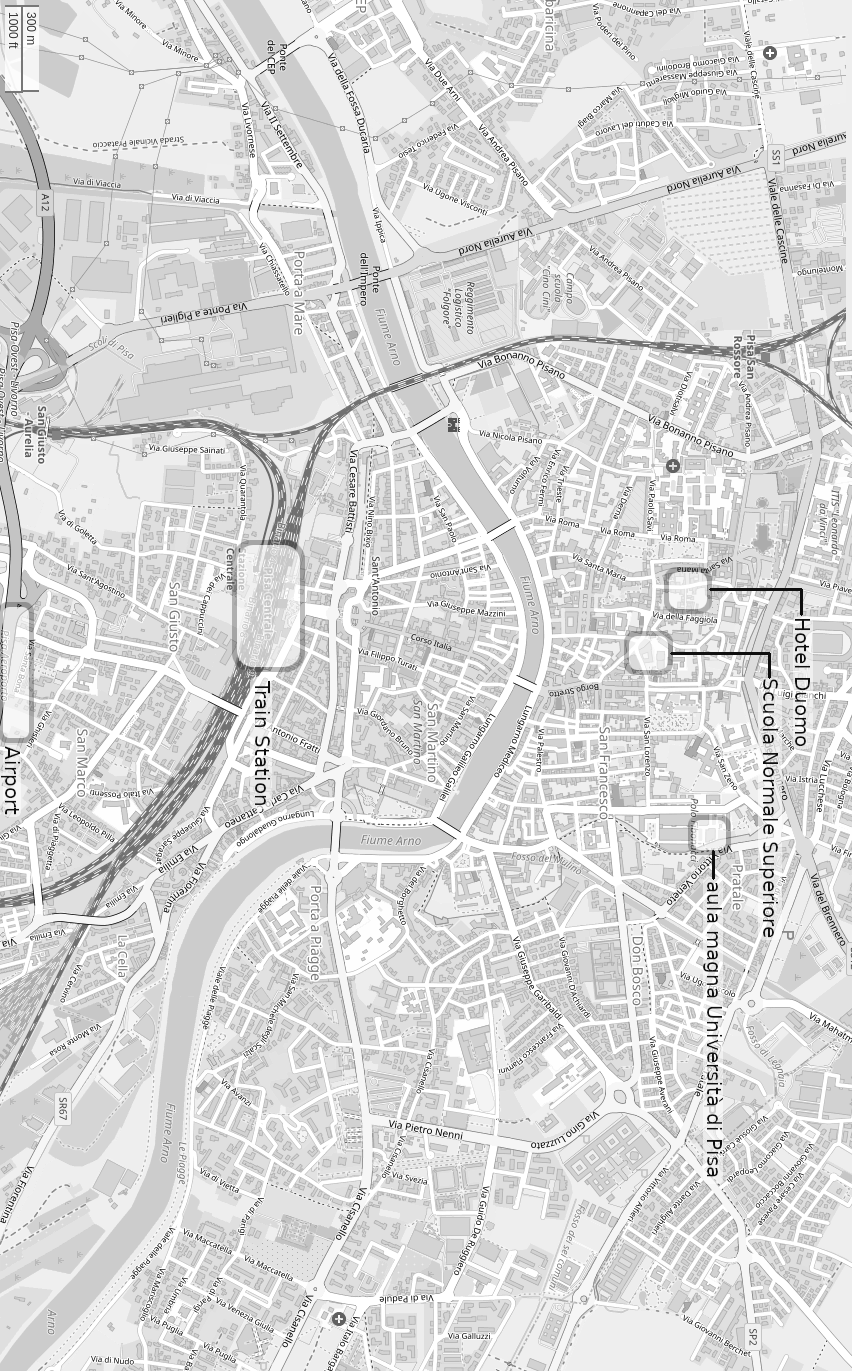
\includegraphics[width=\textwidth]{mappa.png}

\end{document}